\documentclass[11pt]{article}
\usepackage[margin=1in]{geometry}
\usepackage{amsmath,amssymb,amsthm}
\usepackage{booktabs,graphicx,float,xcolor,microtype,url,hyperref}
\hypersetup{colorlinks=true,linkcolor=blue!55!black,urlcolor=blue!55!black}
\emergencystretch=2em

\newtheorem{theorem}{Theorem}[section]
\newtheorem{lemma}[theorem]{Lemma}
\newtheorem{corollary}[theorem]{Corollary}
\newtheorem{proposition}[theorem]{Proposition}
\newcommand{\R}{\mathbb{R}}
\newcommand{\norm}[1]{\left\lVert #1\right\rVert}
\newcommand{\spr}{\varrho}
\newcommand{\spec}{\operatorname{spec}}
\newcommand{\diag}{\operatorname{diag}}
\newcommand{\argmin}{\operatorname*{arg\,min}}
\newcommand{\Id}{\mathrm{I}}
\newcommand{\ii}{\mathrm{i}}
\newcommand{\Ulfa}{U_{\mathrm{patch}}}
\newcommand{\Ubg}{U_{\mathrm{BG}}}
\newcommand{\Urect}{U_{\mathrm{rect}}}
\newcommand{\Ucmp}{U_{\mathrm{cmp}}}

\title{\textbf{Supplementary Information}\\
Four-Corner Spectral Tuning for Quadratic ADMM\\
with Application to Diffeomorphic Image Registration}
\author{Katherine Xie \qquad Jie Wu \qquad Xiaohui Xie\\
\normalsize Department of Computer Science, University of California, Irvine,
Irvine, California, USA}
\date{}

\begin{document}
\maketitle

\section{Purpose and notation}
This supplement develops the optional noncommuting rate certificates, their
proofs, scaling diagnostics, and implementation details. These constructions
are not used to choose the deployed four-corner parameters. We abbreviate the
alternating direction method of multipliers as ADMM and its over-relaxed form
as oADMM. For symmetric
positive semidefinite $H,G\in\R^{dn\times dn}$ and $\rho>0$, define
\[
C_A(\rho)=(A-\rho\Id)(A+\rho\Id)^{-1},
\]
for any symmetric positive semidefinite $A$, and abbreviate
\[
C_H=(H-\rho\Id)(H+\rho\Id)^{-1},\qquad
C_G=(G-\rho\Id)(G+\rho\Id)^{-1}.
\]
The reduced oADMM error operator is
\begin{equation}
E_{\rho,\alpha}=
\left(1-\frac{\alpha}{2}\right)\Id+\frac{\alpha}{2}C_HC_G,
\qquad 0<\alpha\le2.
\label{eq:E}
\end{equation}
Let nonoverlapping patches $\{\Omega_r\}$ partition the full grid, and define
the full-size direct-sum surrogate
\[
\widetilde H=\bigoplus_r(I_{|\Omega_r|}\otimes H_r),\qquad
\widetilde G=\bigoplus_r(G_r\otimes I_d),
\]
where each $H_r$ and $G_r$ is symmetric positive semidefinite. Let
\[
\delta_H=\norm{H-\widetilde H}_2,\qquad
\delta_G=\norm{G-\widetilde G}_2,\qquad
\delta=\delta_H+\delta_G.
\]
The two surrogate operators commute blockwise. If the symbol endpoints used in
the modal maximization are attained, its exact frozen-patch envelope satisfies
$\Ulfa=\norm{\widetilde E_{\rho,\alpha}}_2$. The notation ``exact'' always
refers to this stated frozen separable model; the full variable-coefficient
registration operator is generally noncommuting.

\section{Additive perturbation certificate}\label{sec:additive}
\subsection{Cayley Lipschitz estimate}
\begin{lemma}[Cayley Lipschitz bound]\label{lem:lipschitz}
For symmetric positive semidefinite $A,B$ and $\rho>0$,
\begin{equation}
\norm{C_A(\rho)-C_B(\rho)}_2
\le\frac{2}{\rho}\norm{A-B}_2.
\label{eq:lipschitz}
\end{equation}
\end{lemma}
\begin{proof}
Writing $C_A=\Id-2\rho(A+\rho\Id)^{-1}$ and using the resolvent identity gives
\[
\begin{aligned}
C_A-C_B
&=2\rho\left[(B+\rho\Id)^{-1}-(A+\rho\Id)^{-1}\right]\\
&=2\rho(A+\rho\Id)^{-1}(A-B)(B+\rho\Id)^{-1}.
\end{aligned}
\]
Both resolvent norms are at most $\rho^{-1}$, proving
\eqref{eq:lipschitz}.
\end{proof}

\begin{theorem}[Additive frozen-patch certificate]\label{thm:additive}
For the direct-sum surrogate defined above and the full variable-coefficient
iteration of the same dimension,
\begin{equation}
\spr(E_{\rho,\alpha})
\le\Ulfa(\rho,\alpha)+\frac{\alpha\delta}{\rho}.
\label{eq:additive}
\end{equation}
No commutativity assumption on $H$ and $G$ is required.
\end{theorem}
\begin{proof}
Since every Cayley transform of a positive semidefinite matrix has norm at most
one,
\[
\begin{aligned}
\norm{C_HC_G-C_{\widetilde H}C_{\widetilde G}}_2
&\le\norm{(C_H-C_{\widetilde H})C_G}_2\\
&\quad+\norm{C_{\widetilde H}(C_G-C_{\widetilde G})}_2\\
&\le\frac{2}{\rho}(\delta_H+\delta_G).
\end{aligned}
\]
Apply \eqref{eq:E}, the triangle inequality, and normality of the separable
direct-sum operator, for which its operator norm equals $\Ulfa$. Any
cross-patch couplings removed from the regularizer are included in $\delta_G$.
\end{proof}

\begin{corollary}[Certified linear rate]
If the right-hand side of \eqref{eq:additive} is below one, then the full
linearized oADMM iteration converges linearly with asymptotic factor no larger
than that value.
\end{corollary}

\subsection{Certificate-aware legacy objective}
For standard ADMM, all scalar frozen-modal factors are nonnegative. A
Let $\mathcal C$ denote the finite set of attained frozen-model curvature--symbol
corners. A certificate-aware diagnostic objective is therefore
\begin{equation}
\mathcal U_1(\rho)=
\max_{c\in\mathcal C}
\frac{\rho^2+h_cg_c}{(\rho+h_c)(\rho+g_c)}
+\frac{\delta}{\rho}.
\label{eq:legacy}
\end{equation}
For two corner branches $c_1=(h_1,g_1)$ and $c_2=(h_2,g_2)$, equality after
denominator clearing is
\[
\rho(A_{12}\rho^2+B_{12})=0,
\]
where
\[
A_{12}=(h_2+g_2)-(h_1+g_1),\qquad
B_{12}=g_1g_2(h_1-h_2)+h_1h_2(g_1-g_2).
\]
On an interval where $c=(h,g)$ is active, stationarity of
\eqref{eq:legacy} gives
\begin{equation}
(h+g)\rho^2(\rho^2-hg)
-\delta(\rho+h)^2(\rho+g)^2=0.
\label{eq:quartic}
\end{equation}
Thus the legacy standard-ADMM bound can also be minimized over a finite set of
endpoints, branch intersections, and active quartic roots. This diagnostic is
not the deployed four-corner selector: the additive term often moves its
minimizer toward an unhelpful boundary.

For an admissible interval
$[\alpha_-,\alpha_+]\subset(0,2]$, let $a$ and $b$ be the active minimum and
maximum frozen-modal $\theta$ values at the selected penalty. The
certificate-aware relaxation objective is
\[
F(\alpha)=
\max\{|1-\alpha+\alpha a|,\ |1-\alpha+\alpha b|\}
+\frac{\alpha\delta}{\rho}.
\]
It is convex and piecewise linear. A minimizer belongs to
\[
\left\{
\alpha_-,\alpha_+,\frac{1}{1-a},\frac{1}{1-b},
\frac{2}{2-a-b}
\right\}\cap[\alpha_-,\alpha_+].
\]
Only finite, defined breakpoints are retained. If $b=1$, the modal maximum is
identically one on $(0,2]$, so
$F(\alpha)=1+\alpha\delta/\rho$. Its minimizer is $\alpha_-$ when
$\delta>0$, and every admissible $\alpha$ is optimal when $\delta=0$.

\section{Exact-regularizer block structure}\label{sec:block}
The additive certificate replaces both operators. Sharper bounds retain the
regularizer exactly. Let
\[
G=G_0\otimes I_d,\qquad
K_\rho=(G_0-\rho I_n)(G_0+\rho I_n)^{-1},
\]
so $C_G=K_\rho\otimes I_d$. Write
\[
C_H=\diag(C_1,\ldots,C_n),\qquad
C_i=(H_i-\rho I_d)(H_i+\rho I_d)^{-1}.
\]
Then the $(i,j)$ block of $M:=C_HC_G$ is
\begin{equation}
M_{ij}=(K_\rho)_{ij}C_i.
\label{eq:block_M}
\end{equation}
Although $K_\rho$ and every $C_i$ are symmetric, $M$ is generally nonnormal
because the $C_i$ vary.

\section{Block-Gershgorin disks}\label{sec:gershgorin}
\begin{theorem}[Block-Gershgorin enclosure]\label{thm:gershgorin}
Every eigenvalue of $M=C_HC_G$ lies in a disk
\begin{equation}
\left|z-(K_\rho)_{ii}c_{i,r}\right|
\le \norm{C_i}_2\sum_{j\ne i}|(K_\rho)_{ij}|
\label{eq:bg_disk}
\end{equation}
for some pixel $i$ and eigenvalue $c_{i,r}$ of $C_i$. Consequently
\begin{equation}
\begin{aligned}
\Ubg(\rho,\alpha)=\max_{i,r}\Big[
&\left|1-\frac{\alpha}{2}
+\frac{\alpha}{2}(K_\rho)_{ii}c_{i,r}\right|\\
&+\frac{\alpha}{2}\norm{C_i}_2
\sum_{j\ne i}|(K_\rho)_{ij}|
\Big]
\end{aligned}
\label{eq:Ubg}
\end{equation}
is a rigorous upper bound on $\spr(E_{\rho,\alpha})$.
\end{theorem}
\begin{proof}
Let $Mx=zx$ and choose a block $x_i$ of maximum Euclidean norm. The $i$th
block equation is
\[
\left(zI_d-(K_\rho)_{ii}C_i\right)x_i
=\sum_{j\ne i}(K_\rho)_{ij}C_ix_j.
\]
The diagonal block is normal, so its smallest singular value is the distance
from $z$ to its spectrum. Taking norms, using
$\norm{x_j}\le\norm{x_i}$, and cancelling $\norm{x_i}$ gives
\eqref{eq:bg_disk}. The affine map from $M$ to $E_{\rho,\alpha}$ maps each disk
to the bound \eqref{eq:Ubg}.
\end{proof}

\section{Signed rectangle and commutator information}\label{sec:rectangle}
Decompose
\[
S=\frac{M+M^\top}{2},\qquad Q=\frac{M-M^\top}{2}.
\]
For $i\ne j$,
\[
S_{ij}=(K_\rho)_{ij}\frac{C_i+C_j}{2},\qquad
Q_{ij}=(K_\rho)_{ij}\frac{C_i-C_j}{2}.
\]
Define zero-diagonal symmetric comparison matrices by
\begin{equation}
B^S_{ij}=|(K_\rho)_{ij}|
\norm{(C_i+C_j)/2}_2,\qquad
B^Q_{ij}=|(K_\rho)_{ij}|
\norm{(C_i-C_j)/2}_2,
\label{eq:comparison_matrices}
\end{equation}
and let $d_i^-$ and $d_i^+$ be the extreme eigenvalues of the diagonal block
$(K_\rho)_{ii}C_i$. The block-row quantities are
\begin{align}
m_\rho^{\rm row}
&=\min_i\left[d_i^--\sum_{j\ne i}B^S_{ij}\right],\\
M_\rho^{\rm row}
&=\max_i\left[d_i^++\sum_{j\ne i}B^S_{ij}\right],\\
\eta_\rho^{\rm row}
&=\max_i\sum_{j\ne i}B^Q_{ij}.
\end{align}

\begin{theorem}[Commutator-aware signed rectangle]\label{thm:rectangle}
With $W(M)=\{x^*Mx:\norm{x}_2=1\}$ denoting the numerical range,
\[
W(M)\subset
[m_\rho^{\rm row},M_\rho^{\rm row}]
+\ii[-\eta_\rho^{\rm row},\eta_\rho^{\rm row}].
\]
Therefore
\begin{equation}
\spr(E_{\rho,\alpha})\le
\Urect:=
\max_{x\in\{m_\rho^{\rm row},M_\rho^{\rm row}\}}
\sqrt{\left(1-\frac{\alpha}{2}+\frac{\alpha x}{2}\right)^2
+\left(\frac{\alpha\eta_\rho^{\rm row}}{2}\right)^2}.
\label{eq:Urect}
\end{equation}
\end{theorem}
\begin{proof}
For any normalized complex vector $x$, set $z=x^*Mx$. Then
\[
\operatorname{Re}z=x^*Sx,\qquad
\ii\operatorname{Im}z=x^*Qx.
\]
Hermitian block-Gershgorin bounds applied to $S$ put the first quantity in the
stated real interval. The symmetric matrix of block norms bounds
$\norm{Q}_2$ by its maximum row sum, giving
$|\operatorname{Im}z|\le\eta_\rho^{\rm row}$. Applying the affine map in
\eqref{eq:E} and maximizing the Euclidean modulus over a rectangle gives
\eqref{eq:Urect}; convexity puts the real-coordinate maximum at an endpoint.
\end{proof}

For fixed $\rho$, the squared expressions under the maximum in
\eqref{eq:Urect} are quadratics in $\alpha$. Their minimum is attained at an
admissible interval endpoint, a stationary point of either quadratic, or their
intersection
\[
\alpha=\frac{4}{2-m_\rho^{\rm row}-M_\rho^{\rm row}}
\]
when admissible. This finite conditional selection is useful for analyzing a
certificate but is not used in one-shot registration tuning.

\section{Perron comparison rectangle}\label{sec:perron}
The row maxima can be replaced by global scalar eigenproblems.
\begin{theorem}[Perron comparison]\label{thm:perron}
The signed rectangle theorem remains valid with
\begin{equation}
\begin{aligned}
m_\rho&=\lambda_{\min}\left(\diag(d^-)-B^S\right),\\
M_\rho&=\lambda_{\max}\left(\diag(d^+)+B^S\right),\\
\eta_\rho&=\spr(B^Q).
\end{aligned}
\label{eq:perron}
\end{equation}
These bounds are no weaker than their block-row counterparts. Denote the
resulting value of \eqref{eq:Urect} by $\Ucmp$.
\end{theorem}
\begin{proof}
Partition a complex block vector $x$ and set $y_i=\norm{x_i}_2$. For the
symmetric
part,
\[
x^*Sx
\le\sum_i d_i^+y_i^2
+2\sum_{i<j}B^S_{ij}y_iy_j
=y^\top(\diag(d^+)+B^S)y.
\]
The analogous lower estimate uses $\diag(d^-)-B^S$. Rayleigh--Ritz yields the
first two bounds. Blockwise comparison for the skew part gives
\[
\norm{Qx}_2\le\norm{B^Qy}_2,
\]
and hence
$\norm Q_2\le\norm{B^Q}_2=\spr(B^Q)$ because $B^Q$ is symmetric and
entrywise nonnegative. Finally, extremal eigenvalues and spectral radii of the
comparison matrices are bounded by their maximum absolute row sums, proving
dominance over the row construction.
\end{proof}
The comparison method requires three symmetric scalar $n\times n$ extremal
eigenproblems and does not form the full $dn\times dn$ oADMM matrix.

\section{Sparse truncated-kernel certificate}\label{sec:truncated}
Under periodic boundaries, $K_\rho$ is convolution by a scalar discrete kernel
$k_\rho(s)$. Let $\mathcal R=-\mathcal R$ be a retained finite symmetric set of
offsets containing zero, and define $K_{\rho,\mathcal R}$ as convolution by
$k_\rho(s)\mathbf 1_{\{s\in\mathcal R\}}$. Define
\[
\tau_{\mathcal R}=\sum_{s\notin\mathcal R}|k_\rho(s)|.
\]
Let $M_{\mathcal R}=C_H(K_{\rho,\mathcal R}\otimes I_d)$. Construct the Perron
comparison matrices using retained offsets only and let $U_{\mathcal R}$ be the
resulting affine numerical-range rectangle bound from
Theorem~\ref{thm:perron}.

\begin{corollary}[Truncated convolution certificate]\label{cor:truncated}
\begin{equation}
\spr(E_{\rho,\alpha})
\le U_{\mathcal R}
+\frac{\alpha}{2}\max_i\norm{C_i}_2\,\tau_{\mathcal R}.
\label{eq:truncated}
\end{equation}
\end{corollary}
\begin{proof}
Young's convolution inequality gives
\[
\norm{K_\rho-K_{\rho,\mathcal R}}_2\le\tau_{\mathcal R}.
\]
Write $M=M_{\mathcal R}+D$. Left multiplication by $C_H$ gives
\[
\norm D_2\le\max_i\norm{C_i}_2\,\tau_{\mathcal R}.
\]
For a normalized eigenvector $x$ of $M$ with eigenvalue $z$,
$z=x^*M_{\mathcal R}x+x^*Dx$. The retained numerical-range rectangle bounds
\[
\left|1-\frac{\alpha}{2}
+\frac{\alpha}{2}x^*M_{\mathcal R}x\right|
\le U_{\mathcal R},
\]
while $|x^*Dx|\le\norm D_2$. The triangle inequality yields
\eqref{eq:truncated}.
\end{proof}
For fixed truncation radius, the comparison matrices are sparse. The kernel
can be evaluated by fast Fourier transform (FFT) in $O(n\log n)$ time and extremal comparison
eigenvalues can be estimated matrix-free. The bound is rigorous at every
radius, including zero; usefulness depends on tightness.

\section{Commutator and orientation diagnostics}\label{sec:commutator}
The resolvent identity also yields a direct commutator estimate.
\begin{proposition}[Cayley commutator bound]
\begin{equation}
\norm{[C_H,C_G]}_2
\le
\frac{4\rho^2\norm{[H,G]}_2}
{(\lambda_{\min}(H)+\rho)^2
(\lambda_{\min}(G)+\rho)^2}.
\label{eq:commutator}
\end{equation}
\end{proposition}
\begin{proof}
Use
$C_H=\Id-2\rho(H+\rho\Id)^{-1}$ and the identity
\[
[(H+\rho\Id)^{-1},(G+\rho\Id)^{-1}]
=(H+\rho\Id)^{-1}(G+\rho\Id)^{-1}
[H,G](G+\rho\Id)^{-1}(H+\rho\Id)^{-1},
\]
up to the equivalent ordering convention for the commutator, and then bound
the four resolvents by their smallest shifted eigenvalues.
\end{proof}

For registration,
\[
[H,G]_{ij}=(G_0)_{ij}(H_i-H_j),
\]
so local coefficient differences control noncommutativity. For the rank-one
model and nonzero gradients, set
$\widehat q_i=q_i/\norm{q_i}_2$ and
$P_i=\widehat q_i\widehat q_i^\top$. The sign-invariant orientation difference
between two rank-one Hessians is
\[
\norm{P_i-P_j}_2
=\sqrt{1-(\widehat q_i^\top\widehat q_j)^2}
=|\sin(\phi_i-\phi_j)|,
\]
where orientation angles are taken modulo $\pi$. This projector metric, unlike
$|\sin((\phi_i-\phi_j)/2)|$, is invariant under either sign change
$q_i\mapsto-q_i$. For the controlled study, we additionally compute
\[
\chi=\frac{\norm{HG-GH}_2}{\norm H_2\norm G_2}.
\]
Across the ten cases, $\chi$ ranges from $0.012$ to $0.239$ and has a
descriptive Pearson correlation of $0.87$ with spectral-radius regret.

\section{Certificate experiments and scaling}\label{sec:certificate_results}
\subsection{Structured enclosure comparison}
The controlled suite contains 18 cases. Here $\spr_{\rm act}$ is the true
spectral radius at the selected parameters, $\spr_{\rm ora}$ is the radius at
numerically oracle-optimized parameters, and $U$ is the stated rigorous
enclosure at the selected pair. The enclosure gap is
$(U-\spr_{\rm act})/\spr_{\rm act}$ and the spectral-radius regret is
$(\spr_{\rm act}-\spr_{\rm ora})/\spr_{\rm ora}$. A collapse denotes selection
at the boundary of the admissible set.
\begin{table}[H]
\centering
\caption{Controlled structured-envelope results; medians over 18 cases.}
\begin{tabular}{lrrr}
\toprule
Method & Enclosure gap & Oracle regret & Collapses\\
\midrule
Block resolvent & 0.166 & 0.926 & 6\\
Block Gershgorin & 0.644 & 0.560 & 0\\
Commutator rectangle & 0.602 & 0.431 & 0\\
Comparison rectangle & 0.595 & 0.386 & 0\\
\bottomrule
\end{tabular}
\end{table}
Every enclosure contained the exact radius. Minimizing the additive bound
produced over-conservative relaxation and collapsed in six of 18 cases. The
Perron rectangle retained sign information and had the smallest oracle regret
among the signed constructions, but was still too loose for online tuning.

\begin{figure}[H]
\centering
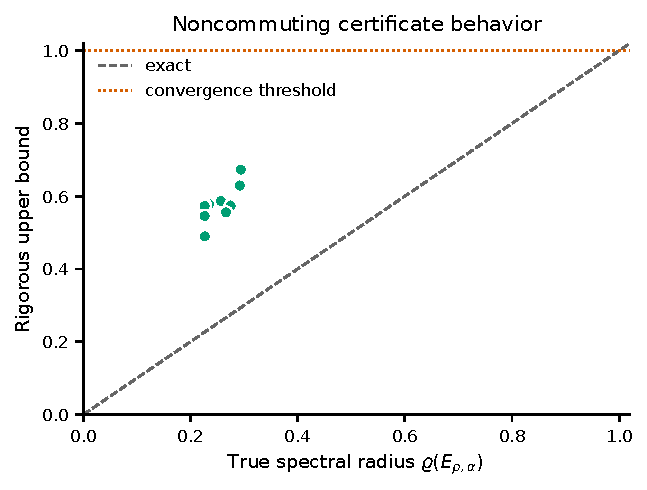
\includegraphics[width=.62\linewidth]{../figures/certificate_behavior.pdf}
\caption{Representative noncommuting certificate values compared with the true
spectral radius on the tractable controlled systems. The bounds remain above
the exact values but are conservative.}
\label{fig:certificate_behavior}
\end{figure}

\subsection{Controlled variable-coefficient predictor tests}
The ten $3\times3$ cases comprise periodic magnitude-only variation,
orientation-only variation, one $90^\circ$ orientation interface, and three
random-gradient stress tests. The latter begin with one fixed periodic
Gaussian white-noise field, apply Gaussian filters with
$\sigma\in\{0.6,1.0,1.6\}$ pixels, differentiate, and rescale each gradient
field to root-mean-square magnitude $0.4$. The filtering scale therefore
describes the precursor scalar field, not monotone smoothness of the normalized
rank-one Hessian. These cases vary gradient magnitude and orientation jointly.

The four-corner predictor attained median spectral-radius regret $0.057$ over
all cases, with no collapse. Regret was $0.003$--$0.087$ for the
single-factor magnitude and orientation constructions, $0.193$ for the abrupt
interface, and $0.238$--$0.296$ for the random-gradient fields. Their
normalized commutators were respectively $0.012$--$0.139$, $0.166$, and
$0.171$--$0.239$. At the selected parameters, the median absolute
relative discrepancy between the four-corner envelope and the true radius was
$1.4\times10^{-15}$, with maximum $2.8\times10^{-3}$. The latter is a
pointwise comparison and does not imply that the surrogate and true spectral
objectives have the same minimizer. The Perron comparison certificate was
below one in all ten cases. Its median enclosure gap was $1.29$, establishing
validity while illustrating conservatism.

\subsection{Truncation scaling}
The truncated-kernel certificate showed no violation in 20 tests spanning
$8^2$ through $64^2$ grids and five truncation radii. Actual matrix-free
spectral radii were approximately $0.269$, while certificate values ranged from
$0.638$ to $0.681$, corresponding to relative gaps $1.38$--$1.54$. The most
expensive $64^2$ retained-radius case took $81.4$ seconds on a central
processing unit (CPU). A relaxed
$128^2$ Arnoldi certificate run did not complete within its allocated
diagnostic window. The sparse representation scales in principle, but the
current eigensolver and bounds are not practical registration-time
certificates.

\subsection{Additional algebraic verification}
Ten thousand randomized curvature configurations were used to compare explicit
pixelwise curvature enumeration with the four-corner envelope. No discrepancy
was observed. Constant-coefficient periodic systems matched the full reduced
spectral radius to numerical precision. These tests validate the implementation
of the separable theorem; they do not turn the variable-coefficient predictor
into an exact global spectral method.

\section{Implementation and baseline details}\label{sec:implementation}
\subsection{Solver}
All methods use the same three-level image pyramid, initialization,
linearization, stopping tolerances, interpolation, line search, and
discrete-Jacobian safeguards. Pixelwise data solves use the
Sherman--Morrison formula; regularizer solves use FFT diagonalization. The line
search requires objective decrease and a discrete-Jacobian floor of $0.05$.
When pyramid upsampling violates this floor, only the nontranslational
displacement is halved until the check passes. This numerical safeguard does
not constitute a global diffeomorphism theorem.

\subsection{Baselines}
The external fixed comparator $(\rho,\alpha)=(0.1,1.0)$ was selected using the
controlled public-image pilot, not FIRE or CIMA, and was then frozen. Residual
balancing starts at $\rho=1$, updates the penalty from primal and dual residual
imbalance, and rescales the dual variable. The Barzilai--Borwein (BB)
comparison is a safeguarded penalty proxy with clipping and periodic updates. Fixed
oADMM uses $(1,1.8)$, while canonical fixed ADMM uses $(1,1)$. Exact update
intervals and safeguards are implemented in
\texttt{src/registration2d.py}.

\subsection{Patch and symbol construction}
Optional certificate studies use fixed, multiresolution, or adaptively split
patches. A representative $\bar q_r$ may be a center, mean, or robust spatial
median, and
\[
H_r=\nu I_d+\mu\bar q_r\bar q_r^\top.
\]
For a direct block surrogate,
\[
\delta_H=\max_i
\norm{\mu q_iq_i^\top+\nu I_d-H_{r(i)}}_2.
\]
Periodic or cosine closures provide analytic regularizer endpoints. For an
order-$p$ Sobolev regularizer,
\[
g(\xi)=
\left(
\gamma+\frac{4\beta}{(\Delta x)^2}
\sum_{\ell=1}^d\sin^2(\xi_\ell/2)
\right)^p,
\]
so
\[
g_-=\gamma^p,\qquad
g_+=\left(\gamma+\frac{4\beta d}{(\Delta x)^2}\right)^p.
\]

\section{Additional benchmark information}\label{sec:benchmark}
\subsection{Controlled real-content pilot}
A public-domain retinal image and an unrestricted immunohistochemistry image
were each subjected to five smooth known deformations. Cases 1--2 selected the
single external fixed comparator; held-out cases 3--5 were not used for tuning and
gave six image--deformation tests. Across five order-alternated repeats (30
paired runs), one-shot tuning reduced median inner
iterations by 44.4\% and median total time by 41.7\% (bootstrap 95\% interval
$[40.9,42.6]$\%). Selection consumed 1.58\% of proposed runtime, median
relative mean squared error (MSE) change was $-0.0068$\%, and no tested case had a nonpositive
Jacobian.

\begin{table}[H]
\centering
\caption{Controlled real-content pilot against the predeclared acceptance
gates; medians over paired runs.}
\begin{tabular}{lrr}
\toprule
Metric & Observed & Gate\\
\midrule
Inner-iteration reduction & 44.4\% & $\ge15$\%\\
Total-time reduction & 41.7\% & $\ge10$\%\\
Relative MSE change & $-0.0068$\% & $\le1$\%\\
Selection overhead & 1.58\% & $<2$\%\\
Nonpositive Jacobians & 0/6 & 0\\
\bottomrule
\end{tabular}
\end{table}

\subsection{Coarse direct spectral optimization diagnostic}
For each CIMA pair, a variable-coefficient reduced operator was assembled on an
$8\times8$ downsampled grid and its penalty was optimized numerically. At each
trial $\rho$, if $\{\lambda_j(\rho)\}$ are the eigenvalues of
$C_H(\rho)C_G(\rho)$, the conditional relaxation was computed from
\[
\alpha_\rho\in\argmin_{10^{-6}\le\alpha\le2}
\max_j\left|1-\frac{\alpha}{2}
+\frac{\alpha}{2}\lambda_j(\rho)\right|.
\]
The resulting pair was transferred to the full $256^2$ registration. The
coarse spectral search required a median 97 spectral-objective evaluations and
$2.18$ seconds of parameter-selection time. Median full-solve iterations were
251, compared with 210 for four-corner tuning, and total times were $4.39$ and
$2.02$ seconds, respectively; target registration error (TRE) was
indistinguishable. This diagnostic quantifies repeated spectral-evaluation
overhead on a tractable surrogate. Parameter transfer from a coarse operator
is distinct from direct spectral optimization of the full-resolution
variable-coefficient system.

\subsection{CIMA preprocessing and initialization}
The public lung-lesion-3 sample comprises five differently stained sections
and all ten unordered pairs. Images supplied at 5\% scale were converted to a
common structural channel by grayscale conversion, contrast-limited adaptive
histogram equalization (CLAHE), Sobel-magnitude extraction, Gaussian smoothing,
and fixed percentile normalization, and were then resized to $256^2$. Manual
landmarks supplied at 50\% scale were rescaled geometrically and used only for
evaluation. Each method used the same image-only robust translation
initialization selected from phase correlation, centroid alignment, and
clustered scale-invariant feature transform (SIFT) proposals on a $128^2$
image.

\subsection{FIRE parameter summary}
The audited FIRE result contains 134 pairs and five methods per pair. Percentage
reductions are computed pairwise before aggregation. For one-shot four-corner
tuning, median $\rho_{\rm 4C}=0.1008$ (interquartile range (IQR) $0.0397$,
range $0.0688$--$0.1402$) and median $\alpha_{\rm 4C}=1.5699$ (IQR $0.1287$, range
$1.4483$--$1.6883$). The median $h_+$ is $0.2249$.

\subsection{One-shot reuse}
On a balanced 18-pair FIRE subset, per-level retuning reduced median inner
iterations from 243 to 222 but increased median tuning time from $0.030$ to
$0.110$ seconds and median total time from $2.651$ to $3.895$ seconds.
Accordingly, all headline experiments use one-shot reuse. Retuning at every
outer Gauss--Newton iteration was not tested separately.

\section{Reproducibility and availability}
The audited runs began at commit
\texttt{3dc78db3013b9ab2eed80f00b04d4455bc809a55} on 6 August 2026 and used
seed 20260806 and \texttt{configs/real2d\_v1.yaml}. The environment used
Python 3.10.9, NumPy 2.2.6, SciPy 1.15.3, pandas 2.3.3,
Matplotlib 3.10.9, and scikit-image 0.25.2 on two Intel Xeon Gold 5218 CPUs;
the experiments were CPU-only. Timed registrations used one Basic Linear
Algebra Subprograms (BLAS)/OpenMP thread.
Exact commands and the complete validation sequence are recorded in
\texttt{results/real2d\_v1/reproducibility\_log.md}. Raw pair-level outputs,
result schemas, and regeneration scripts are stored alongside that log. FIRE
preprocessing uses a foreground-percentile-normalized green channel; CIMA uses
the structural-channel processing described above. Supplied landmarks are used only for
evaluation.

FIRE and CIMA are public datasets subject to their original licenses. Raw FIRE
images are not redistributed. Preparation scripts, integrity checks, all
nonrestricted pair-level measurements, and the certificate implementations
(\texttt{src/structured\_envelopes.py} and the corresponding
\texttt{experiments/} scripts) are available at
\url{https://github.com/xhxuciedu/admm-registration}.

\end{document}
